\documentclass{report}

%packages
\usepackage[utf8]{inputenc}
\usepackage{listings}
\usepackage{courier}
\usepackage{lipsum}
\usepackage{minted}
\usepackage{tabu}
\usepackage{graphicx}
\usepackage{longtable}
\usepackage{caption}

\graphicspath{ {screenshots/} }

\title{Programming Coursework Report}
\author{Quinn Stevens}
\date{June 2017}

\setminted{breaklines}

\begin{document}
\tabulinesep=1.2mm
\maketitle

\tableofcontents

    \part{Quiz Game}
    \chapter{Testing Plan}
    
    \begin{longtable}[c]{|p{0.2\textwidth}|p{0.2\textwidth}|p{0.2\textwidth}|p{0.2\textwidth}|p{0.2\textwidth}|}
    	\hline
        \textbf{Environment} & \textbf{Action} & \textbf{Expected Result} & \textbf{Actual Result} & \textbf{Proof}\\
        \hline
        Program Closed & Run Program & Main Menu form opens & Main Menu form opened & see screenshot \ref{fig:screenshot01}\\
        \hline
        Main Menu & Click 'Quit' Button & Program closes & Program closed & see screenshot \ref{fig:screenshot02}\\
        \hline
        Main Menu & Click 'Easy' Button & Asks first easy question & Asked first easy question & see screenshot \ref{fig:screenshot03}\\
        \hline
        Quiz & Click radio button & Radio button selected & Radio button selected & see screenshot \ref{fig:screenshot04}\\
        \hline
        Quiz & Click Answer while radio button selected & Ask next question & Asked next question & see screenshot \ref{fig:screenshot05} \\
        \hline
        Quiz & Click Answer while radio button not selected & Ask next question & Asked next question & see screenshot \ref{fig:screenshot06} \\
        \hline
        Quiz & Click Skip & Ask Next Question & Asked next question & see screenshot \ref{fig:screenshot07}\\
        \hline
        Quiz & Finish Quiz & Ask if you want to repeat skipped questions & Asked if you want to repeat skipped questions & see screenshot \ref{fig:screenshot08}\\
        \hline
        Skipped Questions Dialogue & Click `Yes' & Re-ask skipped questions & Re-asked skipped questions & see screenshot \ref{fig:screenshot09}\\
        \hline
        Quiz & Finish Quiz with wrong answers (No skipped questions or click `No' on skipped questions dialogue or finished retrying skipped questions) & Show end of quiz report with corrections & Showed end of quiz report with corrections & see screenshot \ref{fig:screenshot10}\\
        \hline
        Quiz & Finish Quiz with no wrong answers & Show end of quiz report without corrections & Showed end of quiz report without corrections & see screenshot \ref{fig:screenshot11}\\
        \hline
        Main Menu & Click `Hard' Button & Asks first hard question & Asked first hard question & see screenshot \ref{fig:screenshot12}\\
        \hline
    \end{longtable}
    
    \chapter{Testing Screenshots}
    
    \begin{figure}[H]
        \centering
        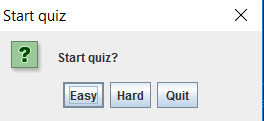
\includegraphics{Screenshot01}
        \caption{Screenshot 01}
        \label{fig:screenshot01}
    \end{figure}
    
    \begin{figure}
        \centering
        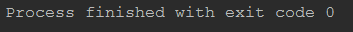
\includegraphics{Screenshot02}
        \caption{Screenshot 02}
        \label{fig:screenshot02}
    \end{figure}
    
    \begin{figure}
        \centering
        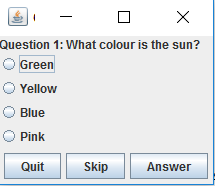
\includegraphics{Screenshot03}
        \caption{Screenshot 03}
        \label{fig:screenshot03}
    \end{figure}
    
    \begin{figure}
        \centering
        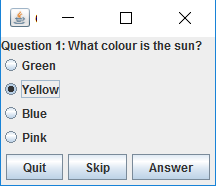
\includegraphics{Screenshot04}
        \caption{Screenshot 04}
        \label{fig:screenshot04}
    \end{figure}

    \begin{figure}
        \centering
        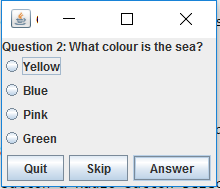
\includegraphics{Screenshot05}
        \caption{Screenshot 05}
        \label{fig:screenshot05}
    \end{figure}
    
    \begin{figure}
        \centering
        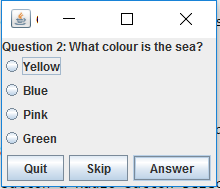
\includegraphics{Screenshot06}
        \caption{Screenshot 06}
        \label{fig:screenshot06}
    \end{figure}
    
    \begin{figure}
        \centering
        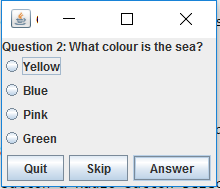
\includegraphics{Screenshot06}
        \caption{Screenshot 07}
        \label{fig:screenshot07}
    \end{figure}
    
    \begin{figure}
    	\centering
    	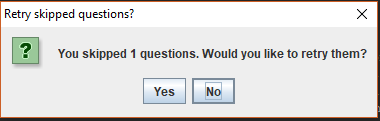
\includegraphics{Screenshot08}
    	\caption{Screenshot 08}
    	\label{fig:screenshot08}
    \end{figure}
    
    \begin{figure}
    	\centering
    	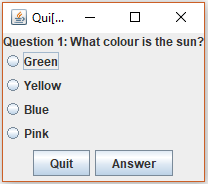
\includegraphics{Screenshot09}
    	\caption{Screenshot 09}
    	\label{fig:screenshot09}
    \end{figure}
    
    \begin{figure}
    	\centering
    	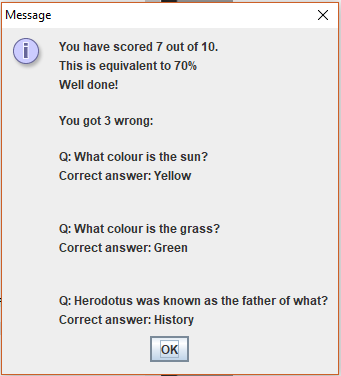
\includegraphics{Screenshot10}
    	\caption{Screenshot 10}
    	\label{fig:screenshot10}
    \end{figure}
    
    \begin{figure}
    	\centering
    	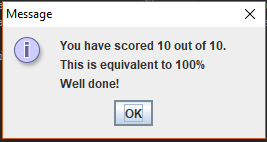
\includegraphics{Screenshot11}
    	\caption{Screenshot 11}
    	\label{fig:screenshot11}
    \end{figure}
    
    \begin{figure}
    	\centering
    	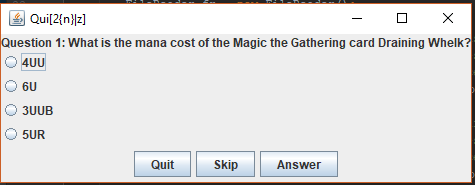
\includegraphics{Screenshot12}
    	\caption{Screenshot 12}
    	\label{fig:screenshot12}
    \end{figure}
    
    \chapter{Critical Analysis}
        \section{Strengths}
        \begin{itemize}
            \item Allows users to choose from two different difficulties
            \item Gives feedback on how the user did
            \item Allows users to save questions for later
        \end{itemize}
        
        \section{Weaknesses}
        \begin{itemize}
            \item Scoring is binary - it doesn't give the user any second chances
            \item Doesn't allow users to skip questions multiple times
            \item Doesn't stop the user if they don't answer a question
        \end{itemize}
        
        \section{Suggested Enhancements}
        \begin{itemize}
        	\item Allow user to skip a question multiple times
        	\item Stop the user from continuing with the quiz if they don't select an answer
        	\item Allow the user to retry questions they got wrong, but with a reduced points reward
        \end{itemize}
        
        \section{Adherence to Specification}
        \begin{longtable}[c]{|p{0.6\textwidth}|p{0.2\textwidth}|}
        	\hline
        	\textbf{Requirement} & \textbf{Fulfilled?} \\ \hline
        	The system should be dialogue-based & Yes \\ \hline
        	Good interface design and programming principles should be applied throughout & Yes \\ \hline
        	Upon start of the program, the first question with its corresponding answers should be displayed & Yes \\ \hline
        	The question number should be displayed, and the options labelled appropriately & Yes \\ \hline
        	When the user clicks the OK button, the second question with its corresponding answers should be displayed & Yes \\ \hline
        	The above step should be repeated until all 10 questions have been displayed & Yes \\ \hline
        	When all questions are answered the program should display the user's score along with an appropriate message & Yes \\ \hline
        	Questions and answers should NOT be hard-coded and must be imported from external files & Yes \\ \hline
        	When taking the test, if the user tries to view the next question without providing an answer to the current question, a message should be displayed to alert them & No \\ \hline
        	In returning to a skipped question, an answer must be provided (A question cannot be skipped twice) & Yes (although I do not agree that this improves the test program) \\ \hline
        	The system should display the questions that have been incorrectly answered. Repeating the failed questions should not change the user's final score. & Yes (again, I believe that changing this would improve the program) \\ \hline
        	The user should have the choice of the difficulty level of the test: e.g. setting up two or more files each containing a set of questions at different levels of difficulty & Yes \\ \hline
        \end{longtable}
    
	\chapter{Source Code}
\begin{minted}{java}
import javax.swing.*;

/**
 * Created by Quinn Stevens on 31/05/2017.
 */
public class Quiz {
    static int score = 0;

    public static void main (String[] args) {
        runQuiz();
    }

    public static void runQuiz() {
        String[] questions;
        String[][] options;
        String[] correctAnswers;

        Object[] difficulties = {"Easy", "Hard", "Quit"};

        int difficulty = JOptionPane.showOptionDialog(null, "Start quiz?", "Start quiz", JOptionPane.YES_NO_OPTION, JOptionPane.QUESTION_MESSAGE, null, difficulties, difficulties[0]);

        FileReader fr = new FileReader();
        if (difficulty == 0) {
            questions = fr.getArray("resources/easy/questions.txt");
            options = fr.getAnswerArray("resources/easy/options.txt");
            correctAnswers = fr.getArray("resources/easy/answers.txt");
            QuestionMaster qm = new QuestionMaster(questions, options, correctAnswers);
        } else if (difficulty == 1){
            questions = fr.getArray("resources/hard/questions.txt");
            options = fr.getAnswerArray("resources/hard/options.txt");
            correctAnswers = fr.getArray("resources/hard/answers.txt");
            QuestionMaster qm = new QuestionMaster(questions, options, correctAnswers);
        } else {
            System.exit(0);
        }
    }
}
\end{minted}
\captionof{listing}{Quiz.java}

\begin{minted}{java}
import javax.swing.*;
import java.awt.*;
import java.awt.event.ActionEvent;
import java.awt.event.ActionListener;
import java.util.Objects;
import java.util.Stack;

/**
 * Created by Quinn Stevens on 31/05/2017.
 */
public class QuestionMaster implements ActionListener {
    JFrame frame;
    int questionNum= 0;
    int score = 0;
    String currentAnswer;

    String[] questions;
    String[][] options;
    String[] answers;

    boolean skipAllowed;
    Stack skipped = new Stack();
    int incorrectAnswers = 0;

    String report = "";

    public QuestionMaster (String[] questions, String[][] options, String[] answers) {
        this.questions = questions;
        this.options = options;
        this.answers = answers;
        this.questionNum = 0;
        skipAllowed = true;
        askQuestion(questions[questionNum], options[questionNum], answers[questionNum]);
    }

    private void askQuestion(String question, String[] options, String answer) {
        frame = new JFrame("Qui[2{n}|z]");
        frame.setDefaultCloseOperation(JFrame.EXIT_ON_CLOSE);
        frame.setLocation(600, 300);
        frame.setLayout(new BorderLayout());

        // Panel for question
        JLabel qLabel = new JLabel("Question " + (questionNum+1) + ": " + question);

        // Panel for answer options
        JPanel buttonPanel = new JPanel(new GridLayout(0, 1));
        ButtonGroup buttonGroup = new ButtonGroup();
        JRadioButton[] answerButtons = new JRadioButton[options.length];
        for (int i = 0; i < answerButtons.length; i++) {
            answerButtons[i] = new JRadioButton(options[i]);
            answerButtons[i].addActionListener(this);
            buttonGroup.add(answerButtons[i]);
            buttonPanel.add(answerButtons[i]);
        }

        // Panel for controls
        JPanel controlPanel = new JPanel(new FlowLayout());
        // Create quit button
        JButton quitButton = new JButton("Quit");
        quitButton.setActionCommand("quit");
        quitButton.addActionListener(this);
        controlPanel.add(quitButton);

        if (skipAllowed) {
            // Create skip button
            JButton skipButton = new JButton("Skip");
            skipButton.setActionCommand("skip");
            skipButton.addActionListener(this);
            controlPanel.add(skipButton);
        }

        // Create submit button
        JButton answerButton = new JButton("Answer");
        answerButton.setActionCommand("answer");
        answerButton.addActionListener(this);
        controlPanel.add(answerButton);

        frame.add(qLabel, BorderLayout.NORTH);
        frame.add(buttonPanel, BorderLayout.CENTER);
        frame.add(controlPanel, BorderLayout.SOUTH);
        frame.pack();
        frame.setVisible(true);
    }

    private void nextQuestion() {
        frame.dispose();
        questionNum++;
        if (questionNum < questions.length) {
            askQuestion(questions[questionNum], options[questionNum], answers[questionNum]);
        } else if (!skipped.empty()) {
            Object[] skipOptions = {"Yes", "No"};
            int retry = JOptionPane.showOptionDialog(
                    null,
                    "You skipped " + skipped.size() + " questions. Would you like to retry them?",
                    "Retry skipped questions?",
                    JOptionPane.YES_NO_OPTION,
                    JOptionPane.QUESTION_MESSAGE,
                    null,
                    skipOptions,
                    skipOptions[1]);
            if (retry == 0) {
                skipAllowed = false;
                retrySkipped();
            } else {
                endQuiz();
            }
        } else {
            endQuiz();
        }
    }

    private void updateReport() {
        incorrectAnswers += 1;
        report += "\n\nQ: " + questions[questionNum] + "\nCorrect answer: " + answers[questionNum] + "\n";
    }

    private void endQuiz() {
        if (incorrectAnswers != 0) {
            report = "\n\nYou got " + incorrectAnswers + " wrong:" + report;
        }

        JOptionPane.showMessageDialog(null, "You have scored " + score + " out of 10.\n" +
                "This is equivalent to " + Math.round(score/10.0*100) + "%\nWell done!" + report);
    }

    private void checkAnswer() {
        if (Objects.equals(currentAnswer, answers[questionNum])) {
            score ++;
        } else {
            updateReport();
        }
    }

    private void resetQuiz() {
        frame.dispose();

        Quiz.runQuiz();
    }

    private void retrySkipped() {
        int stackSize = skipped.size();
        String[] skippedQs = new String[stackSize];
        String[][] skippedOpts = new String[stackSize][4];
        String[] skippedAnsw = new String[stackSize];

        for (int i = stackSize-1; i >= 0; i--) {
            int qNum = (int) skipped.pop();
            skippedQs[i] = questions[qNum];
            skippedOpts[i] = options[qNum];
            skippedAnsw[i] = answers[qNum];
        }

        questions = skippedQs;
        options = skippedOpts;
        answers = skippedAnsw;
        questionNum = -1;
        nextQuestion();
    }

    @Override
    public void actionPerformed(ActionEvent event) {
        String command = event.getActionCommand();

        if (command == "answer" && currentAnswer != null) {
            checkAnswer();
            nextQuestion();
        } else if (command == "answer" && currentAnswer == null) {
            JOptionPane.showMessageDialog(null, "You haven't selected an answer!");
        } else if (command == "quit") {
            resetQuiz();
        } else if (command == "skip") {
            skipped.push(questionNum);
            nextQuestion();
        } else {
            currentAnswer = command;
        }
    }
}
\end{minted}
\captionof{listing}{QuestionMaster.java}

\begin{minted}{java}
import java.io.File;
import java.io.IOException;
import java.util.Scanner;
import java.util.Stack;

/**
 * Created by Quinn Stevens on 31/05/2017.
 */
public class FileReader {
    public String[][] getAnswerArray(String filename) {

        String[] inputArray = getArray(filename);
        String[][] outputArray = new String[inputArray.length][4];
        String[] splitText;
        for (int i = 0; i < inputArray.length; i++) {
            splitText = inputArray[i].split(", ");

            for (int j = 0; j < splitText.length; j++) {
                outputArray[i][j] = splitText[j];
            }
        }

        return outputArray;
    }

    public String[] getArray(String filename) {
        String[] text = null;
        try {
            text = readFile(filename);
        } catch (IOException e) {
            e.printStackTrace();
        }

        return text;
    }

    public static String[] readFile(String filename) throws IOException {
        String fileLine;
        Stack textStack = new Stack();

        File questionFile = new File(filename);
        Scanner fileScan = new Scanner(questionFile);

        while (fileScan.hasNext()) {
            fileLine = fileScan.nextLine();
            textStack.push(fileLine);
        }

        String[] textArray = new String[textStack.size()];

        for (int i = textArray.length -1; i >=0; i--) {
            textArray[i] = (String) textStack.pop();
        }

        return textArray;
    }
}
\end{minted}
\captionof{listing}{FileReader.java}

\addcontentsline{toc}{chapter}{Appendix I: Banking Program}
\chapter*{Appendix I: Banking Program}
\section{Source Code}
\section{Output}
\end{document}
